%There are two main streams of process control - continuous and sequential\cite{dunn2006introduction}. Continuous control involves the constant monitoring and manipulation of dynamic systems while while sequential control is event based. Given the nature of the lolly machine, sequential control is the obvious choice for controlling the system \cite{dunn2006introduction}.

The lolly machine is, in essence, an automatic machine. This section investigates various components that facilitate the automation aspects of the project.

\subsection{Programmable Logic Controller}


    A \acrfull{plc} is an industrial controller/ computer that can be programmed to perform specific \acrshort{rt} tasks and can utilised for varying applications\cite{petruzella2017programmable}. A \acrshort{plc} performs these tasks through solving logic based operations\cite{petruzella2017programmable}.  E.g., if a water tank is filled to a level which is deemed "to high" turn off the water supply to the tank. A \acrshort{plc} interacts with the outside world through the use of either onboard or remote \acrshort{io}.
    
    Prior to the existence of \acrshort{plc}s, sequential based control was performed through relay\footnote{Relays are an electrical component comprised of a solenoid and contacts(\acrshort{no} and/or \acrshort{nc}), when the solenoid is energised the contacts change state.}-logic. Relay logic required multiple relays to be wired in a certain configuration allowing for the control of the system. Figure \ref{fig:relayLogic} shows an example of a relay-logic based control system\cite{petruzella2017programmable}. 
    \acrshort{plc}s provided a much cleaner, organised and easier to troubleshoot method of control as seen in Figure \ref{fig:plcLogic}.    
    
    \begin{figure}[H]
    \centering
    \begin{minipage}{0.35\textwidth}
        \centering
        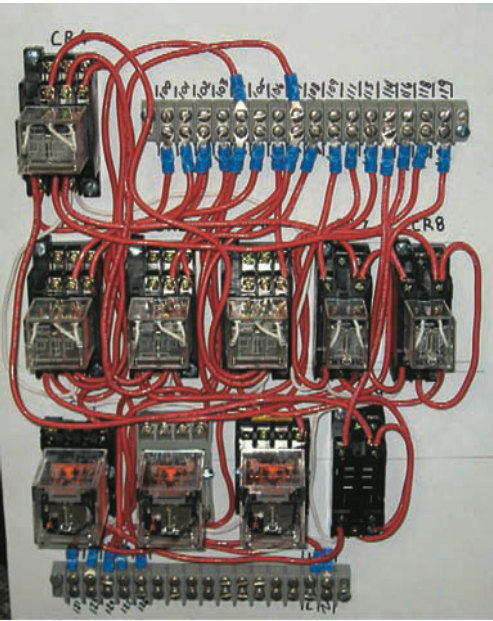
\includegraphics[width = 0.9\textwidth]{2_images/relayLogic.png}
        \caption{Relay logic based control system.~\cite{petruzella2017programmable}}
        \label{fig:relayLogic}
    \end{minipage}\hfill
    \begin{minipage}{0.35\textwidth}
        \centering
        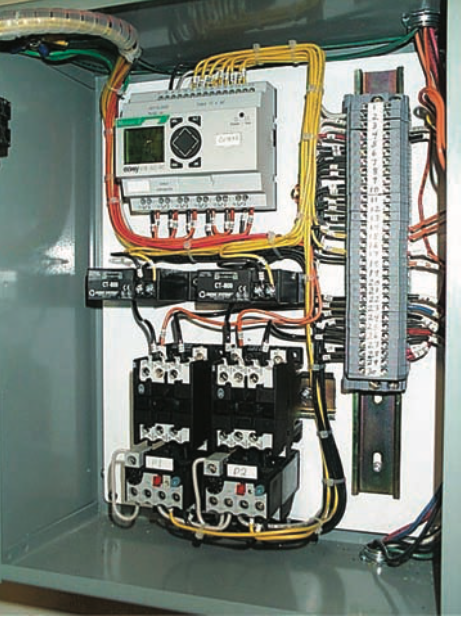
\includegraphics[width = 0.9\textwidth]{2_images/plcLogic.png}
        \caption{\acrshort{plc} based control system.~\cite{petruzella2017programmable}}
        \label{fig:plcLogic}
    \end{minipage}\hfill            
    \end{figure}   
    
    Originally, \acrshort{plc}s where exclusively programmed in a language called \acrfull{ld}\cite{petruzella2017programmable}. Ladder logic is a visual programming language based on electrical control schematics and was designed to be used by the same people who were building the relay logic based control systems ,electricians\cite{petruzella2017programmable}. In more recent times \acrshort{plc}s have become more sophisticated and can be programmed in a variety of languages including \acrfull{st} which is a text based language\cite{petruzella2017programmable}. 
    
    A \acrshort{plc}'s main components are a power supply, \acrlong{cpu}, and \acrshort{io} modules. \acrshort{io} modules can be located locally or remotely. Local \acrshort{io} is physically connected to the \acrshort{plc} while remote \acrshort{io} is connected to the \acrshort{plc} via a communication line, this is illustrated in Figure \ref{fig:localRemoteIo}.
    
    \begin{figure}[H]
        \centering
        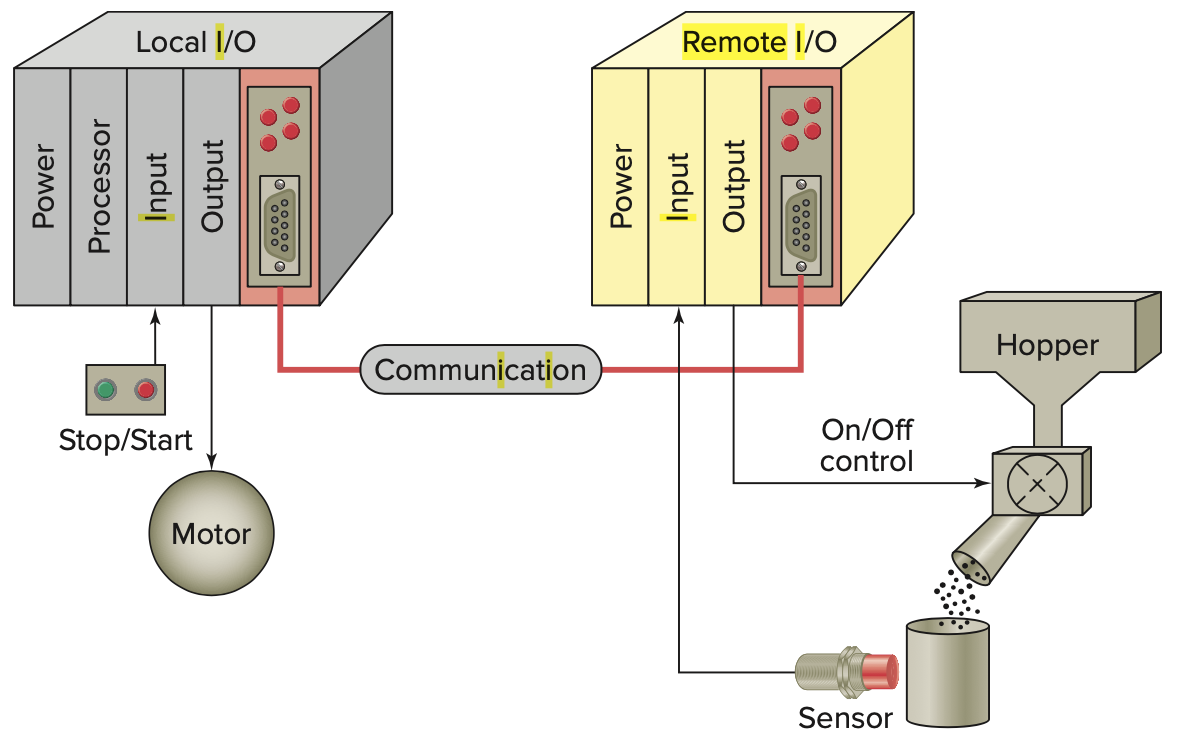
\includegraphics[width = 0.5\textwidth]{2_images/localRemoteIo.png}
        \caption{Local and remote \acrshort{io}}
        \label{fig:localRemoteIo}
    \end{figure}
  
    
\subsection{HMI}
    A \acrfull{hmi}, as the name suggests, is the interface between the machine and the operator. A \acrshort{hmi} is a screen that shows the machine state through graphics. An operator enters commands through the touch screen or a keyboard and mouse. \acrshort{hmi}s are programmable and can be used to control and monitor almost any machine\cite{petruzella2017programmable}. Typically, there is one \acrshort{hmi} per machine/ operator. It is not uncommon to have multiple \acrshort{hmi}s within a single factory. Figure \ref{fig:typHmi} shows an example of what a \acrshort{hmi} screen for a basic motor controller might look like.

    \begin{figure}[H]
        \centering
        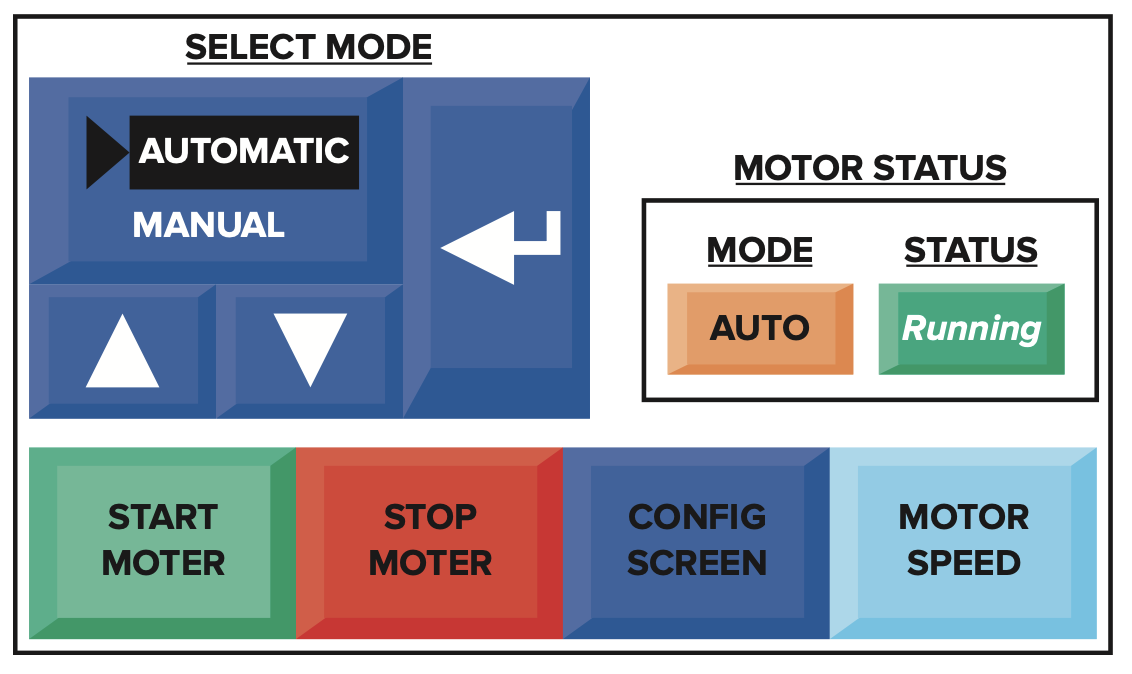
\includegraphics[width = 0.5\textwidth]{2_images/typicalHmi.png}
        \caption{A typical \acrshort{hmi} motor controller screen\cite{petruzella2017programmable}}
        \label{fig:typHmi}
    \end{figure}    
    
\subsection{Engineering Workstation}
    An engineering workstation is a \acrshort{pc} that has been set up for a engineer. The engineering workstation is connected to the \acrshort{ot} network and setup with all relevant software specific to the controlled process.  
\newpage    
\subsection{Microcontrollers}
    To understand what a microcontroller is, a few definitions must be made \cite{crisp2003introduction}.
    
\begin{description}
    \item{Integrated Circuits:} - An electronic circuit that is printed onto solid block. The circuit contains semi-conductor components. Integrated circuits are often referred to as chips.
    \item{Microprocessor:} - A microprocessor is part of a system, it is the central processing unit and is useless without surrounding circuitry and applied voltages.
    \item{Microprocessor-based System:} A microprocessor-based System is any system that is controlled by a microprocessor. 
\end{description}    
    
    A \textbf{microcontroller} is a complete microprocessor-based system built into an integrated circuit and is usually capable of controlling its own \acrshort{io} \cite{crisp2003introduction}.
    
    Microcontrollers are capable of performing an almost infinite list of tasks, e.g., controlling a wrist watch, monitoring and controlling a home irrigation system or controlling a robot. Some micorcontrollers, like the ones in a wrist watch or calculator,  can not be easily programmed after they leave the factory while other can.
    
    Similar to a \acrshort{plc}, micorcontrollers have onboard \acrshort{io} with the caveat being the hyper sensitivity to voltages above the standard operating voltage of the microcontroller which is typically 3.3 volts. Two micorcontrollers are used on the lolly machine - these are a Raspberry Pi and an Arduino.  
  
    \begin{figure}[H]
    \centering
    \begin{minipage}{0.4\textwidth}
        \centering
        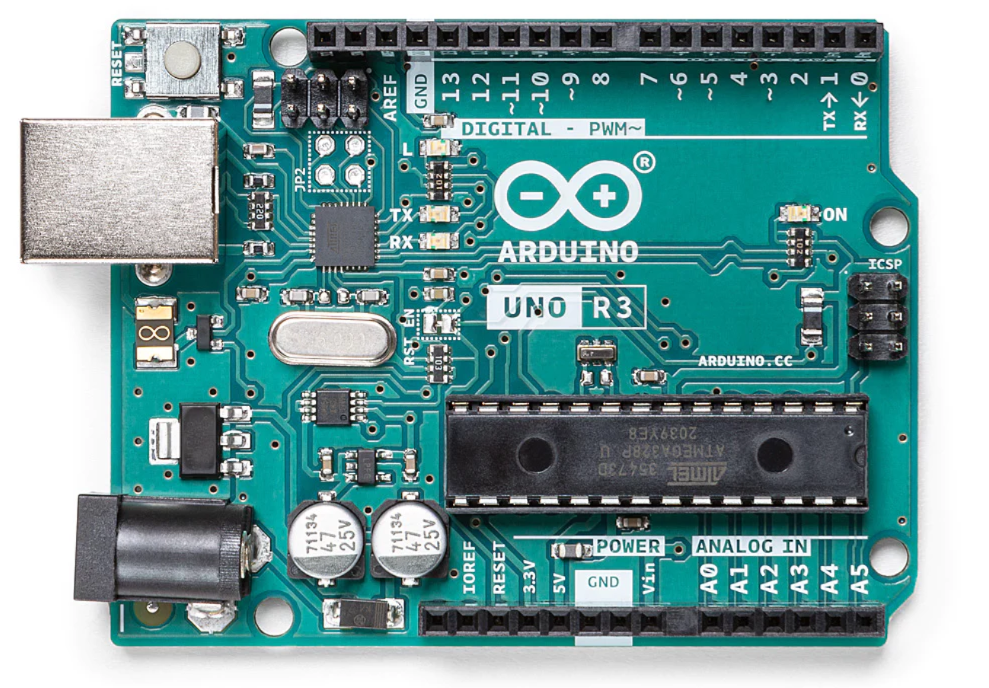
\includegraphics[width = 0.8\textwidth]{2_images/arduino.png}
        \caption{An Arduino~\cite{arduinoWeb}}
        \label{fig:arduino}
    \end{minipage}\hfill
    \begin{minipage}{0.4\textwidth}
        \centering
        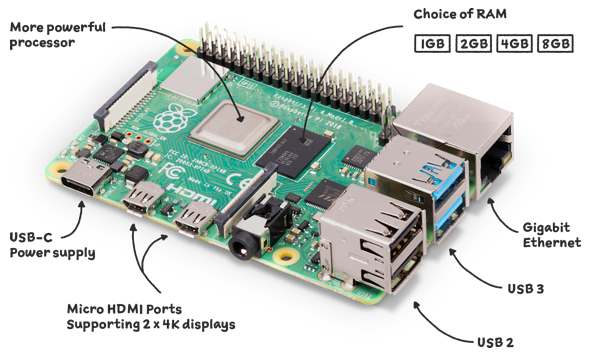
\includegraphics[width = 0.9\textwidth]{2_images/RaspPi.png}
        \caption{A Raspberry Pi~\cite{raspPiWeb}}
        \label{fig:raspPi}
    \end{minipage}\hfill            
    \end{figure}     

        

    
